% CVPR 2022 Paper Template
% based on the CVPR template provided by Ming-Ming Cheng (https://github.com/MCG-NKU/CVPR_Template)
% modified and extended by Stefan Roth (stefan.roth@NOSPAMtu-darmstadt.de)

\documentclass[10pt,twocolumn,letterpaper]{article}

%%%%%%%%% PAPER TYPE  - PLEASE UPDATE FOR FINAL VERSION
%\usepackage[review]{cvpr}      % To produce the REVIEW version
\usepackage{cvpr}              % To produce the CAMERA-READY version
%\usepackage[pagenumbers]{cvpr} % To force page numbers, e.g. for an arXiv version

% Include other packages here, before hyperref.
\usepackage{graphicx}
\usepackage{amsmath}
\usepackage{amssymb}
\usepackage{booktabs}
\usepackage{float}
\usepackage{float} % For positionning images
\usepackage{tabularx} % For tables


% It is strongly recommended to use hyperref, especially for the review version.
% hyperref with option pagebackref eases the reviewers' job.
% Please disable hyperref *only* if you encounter grave issues, e.g. with the
% file validation for the camera-ready version.
%
% If you comment hyperref and then uncomment it, you should delete
% ReviewTempalte.aux before re-running LaTeX.
% (Or just hit 'q' on the first LaTeX run, let it finish, and you
%  should be clear).
\usepackage[pagebackref,breaklinks,colorlinks]{hyperref}


% Support for easy cross-referencing
\usepackage[capitalize]{cleveref}
\crefname{section}{Sec.}{Secs.}
\Crefname{section}{Section}{Sections}
\Crefname{table}{Table}{Tables}
\crefname{table}{Tab.}{Tabs.}


%%%%%%%%% PAPER ID  - PLEASE UPDATE
\def\cvprPaperID{****} % *** Enter the CVPR Paper ID here
\def\confName{CVPR}
\def\confYear{2023}

\begin{document}

%%%%%%%%% TITLE - PLEASE UPDATE
\title{Unmasking Sarcasm - Enhancing Sentiment Analysis in E-Commerce Reviews and Questions
}

\author{Hugo Bouy\\
Illinois Tech\\
{\tt\small hbouy@hawk.iit.edu}
% For a paper whose authors are all at the same institution,
% omit the following lines up until the closing ``}''.
% Additional authors and addresses can be added with ``\and'',
% just like the second author.
% To save space, use either the email address or home page, not both
\and
Rémi Kalbe\\
Illinois Tech\\
{\tt\small rkalbe@hawk.iit.edu}
\and
Mathias Roumane\\
Illinois Tech\\
{\tt\small mroumane@hawk.iit.edu}
}
\maketitle

%%%%%%%%% ABSTRACT
% \begin{abstract}
%    The ABSTRACT is to be in fully justified italicized text, at the top of the left-hand column, below the author and affiliation information.
%    Use the word ``Abstract'' as the title, in 12-point Times, boldface type, centered relative to the column, initially capitalized.
%    The abstract is to be in 10-point, single-spaced type.
%    Leave two blank lines after the Abstract, then begin the main text.
%    Look at previous CVPR abstracts to get a feel for style and length.
% \end{abstract}

%%%%%%%%% BODY TEXT
\section{Problem description}
\label{sec:intro}
In an increasingly e-commerce driven world, the analysis of review, comments and questions written by consumers online has become a field of interests.
Understanding opinions and emotions expressed in product feedback/related questions is essential to enhance the user’s experience.
One aspect that might be overlooked in this area is sarcastic and humor detection that can lead to a misinterpretation of these texts.

Humor remains a complex human phenomenon that is far from having a clear definition.
While humor and sarcastic mechanisms are integral to human interaction, its subjective nature makes it a challenging target for computational analysis.
Recent work has been able to open up this area using deep learning and natural language processing advances.
With this project, we will attempt to improve e-commerce review processing using deep learning models for humor disambiguation.

%-------------------------------------------------------------------------

\section{Brief Survey of Previous Work}

Several studies have been conducted over the past years in the ambition of detecting humor and sarcasm:

Jain et al.~\cite{jain2019} delved into the complexities of identifying sarcasm in Amazon reviews. Recognizing sarcasm is crucial for accurate sentiment analysis, especially since sarcastic comments can be misinterpreted by traditional opinion mining methods. They utilized the "Sarcasm Corpus" containing labeled ironic and regular Amazon reviews, extracting features like sentiment scores, punctuation patterns, and contextual elements that consider the contrast between review sentiment and product rating. Their experiments designated the Support Vector Machine (SVM) classifier as the most accurate, emphasizing the role of context in sarcasm detection.

Building upon the idea of sarcasm detection, Poria et al.~\cite{poria2020} introduced a method using deep convolutional neural networks (CNNs). They critiqued traditional methods that treat sarcasm detection as mere text categorization, arguing that such approaches often miss the deeper understanding of language nuances required for sarcasm. Their method integrates sentiment, emotion, and personality features extracted from pre-trained CNNs. By leveraging Twitter data, they contrasted sarcastic sentences with the ground-truth polarity of events. Their experiments with word embeddings from word2vec and a combined CNN-SVM approach demonstrated superior performance on benchmark datasets.

Yaghoobian et al.~\cite{yaghoobian2020} further discussed the challenges of sarcasm detection in sentiment analysis. They categorized detection methods into content-based, which focus on lexical indicators, and context-based, which emphasize background knowledge. Their study highlighted the CASCADE model, which uses user embeddings to capture user-specific features, as an example of leveraging context for sarcasm detection.

Shifting the focus to humor detection, Ziser et al.~\cite{ziser2020} identified product bias in Product Question Answering (PQA) systems, where certain products attract more humorous questions. They proposed a deep-learning framework to detect humor in PQA, focusing on incongruity and subjectivity.

Annamoradnejad and Zoghi~\cite{annamoradnejad2020} proposed the ColBERT model for humor detection. This model leverages BERT embeddings for sentence representation and has achieved state-of-the-art results on various datasets.

Lastly, Gupta et al.~\cite{gupta2021} explored the potential of Large Language Models (LLMs) in humor detection. Their research emphasized the capability of LLMs to capture the intricacies associated with humor and offense detection.


%-------------------------------------------------------------------------
\section{Datasets}
\subsection{Combined dataset for sarcasm detection}

To train our future models, we built a collection of datasets containing several sarcastic and non-sarcastic text. 
The main datasets used in the scope of this project are listed below.
\begin{itemize}
    \item {\bfseries Headlines dataset \cite{misra2019}}: Contains a list of 28,619 headlines collected from two news websites.
    On one hand, TheOnions aims to produce sarcastic versions of real news events.
    On the other hand, real and non-sarcastic news headlines are collected from HuffPost. This dataset has the advantage of having no spelling mistakes and informal usage since it is written by dedicated professionals in a formal manner.
    \item {\bfseries MUStARD++ dataset \cite{mustard2022}}: Mustard++ is a multimodal sarcasm dataset that has been annotated with 9 emotions.
    It was compiled from popular TV shows such as Friends, The Golden Girls or The Big Bang Theory. We will be using this dataset mostly to detect sarcasm but if we have time we may use the annotation to classify the emotion associated with the sarcastic sentence considered.
    \item {\bfseries Sarcasm Corpus V2 dataset \cite{oraby2016}}: This dataset contains both sarcastic and non-sarcastic utterances.
    They are additionally classified in three different types: generic (6,520 samples), hyperbole (1.164 samples) and rhetorical (1,702 samples).
    \item {\bfseries Sarcasm Amazon reviews dataset \cite{filatova2012}}: Contains a large number of both regular and ironic Amazon reviews.
    Each review is also associated with information about the product for which the review was written, the number of stars assigned by the author, etc.
    This dataset will be the most useful in the second part of our project when we link the sarcastic review with the information regarding the product.
\end{itemize}

\begin{figure}[H]
    \centering
    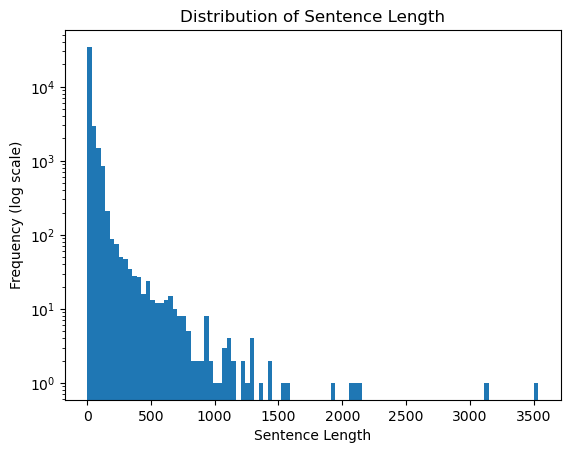
\includegraphics[width=0.8\linewidth]{Figure_sentence_length.png}
    \caption{Frequency of sentence length in the final combined dataset}
    \label[type]{sentence_fig}
\end{figure}

As an initial data processing step, we first concatenated those datasets together in order to use them to implement an initial sarcasm detection model. The final combined dataset then has the full sentence or review and a sarcastic indicator (0 or 1). The final combined dataset contains 40,461 samples from different sources and types. We then have a quite complex dataset with sentences of very variable length as displayed in figure \ref*{sentence_fig}.

\subsection{Amazon reviews dataset}

In order to explore more in depth our problematic around e-commerce, the sarcasm Amazon reviews dataset remains the most useful one in the scope of our project.
As described previously, it contains reviews of products on Amazon that are labelled either as sarcastic or regular. 
Additionally, this dataset reports other information associated to the review such as the product associated with it, the number of stars assigned by the author, etc. 
One of the sampled sarcastic reviews extracted from this dataset is given in table \ref*{tab:mytable} as an example.

\begin{table}[H]
\centering
\small
\begin{tabular}{|c|p{6cm}|}
\hline
\textbf{Feature} & \textbf{Example} \\
\hline
STARS & 3.0 \\
TITLE & Great Product, Poor Packaging \\
DATE & May 14, 2009 \\
AUTHOR & Patrick J. McGovern "Procrastinating Evil Scientist"\\
PRODUCT & Uranium Ore \\
REVIEW & I purchased this product 4.47 Billion Years ago and when I opened it today, it was half empty. \\
\hline

\end{tabular}
\caption{Example of an ironic review sample and the associated information}
\label{tab:mytable}
\end{table}

The additional information offered by this dataset will allow us to take additional parameters into account rather than basing our prediction solely on the review.
We consider that adding these features may help the model to better identify the underlying patterns of sarcasm.






%-------------------------------------------------------------------------
\section{Models}
\subsection{Simple Sarcasm detection model}
As introduced above, we build a heterogeneous dataset with sarcasm examples from very different sources and context.
Our goal here is to experiment building a model that could learn the inner structure of sarcasm from a large amount of data.

Before doing so, and as a starting point for this project, we first aimed at creating a simple model capable of detecting if a sentence contains some from of sarcasm using the Amazon review dataset only.
At this stage, the model only takes into account the sentence and no additional factors. We will later add additional relevant factors in detecting sarcastic or humorous patterns such as information on the product considered.

Jain et al. previously conducted an experiment on this dataset~\cite{jain2019}.
Their idea was to build a feature vector for each Amazon review using various features such as the positive/negative sentiment score, punctuation, part of speech and bigram analysis.
Their results shown very good accuracy with Naïve Bayes (77.50\%), a multi-layer perceptron classifier (81\%), and SVM (81.5\%), with similar precision, recall and f1.
To verify the necessity of this feature selection, we created 2 models, one SVM and one LSTM and train them on plain data, without feature selection.
SVM used count vectorization and the LSTM used word embedding.
Our results showed that SVM performed well with 82\% accuracy on the Amazon review dataset.
However, digging into the results revealed that the model was more likely to misclassify a sarcasm text with both precision and recall being much under the ones for Regular text.
One explanation for this difference may be the small size of the dataset which contains only 1254 texts, with only 437 being sarcastic.

\begin{table}[H]
    \centering
    \begin{tabularx}{\linewidth}{|X|X|X|X|}
        \hline
        & Precision & Recall & F1-score \\
        \hline
        Regular & 0.84 & 0.90 & 0.87 \\
        \hline
        Sarcasm & 0.72 & 0.61 & 0.66 \\
        \hline
    \end{tabularx}
    \caption{Precision, Recall and F1-score for SVM on the Amazon review dataset with only count vectorization.}
\end{table}

The LSTM model on its side less performed with a test accuracy of 67\%.
A Similar behavior can be observed regarding the sarcastic text for which the model fails to understand the sarcasm pattern in all the cases.

\begin{table}[H]
    \centering
    \begin{tabularx}{\linewidth}{|X|X|X|X|}
        \hline
        & Precision & Recall & F1-score \\
        \hline
        Regular & 0.81 & 0.71 & 0.76 \\
        \hline
        Sarcasm & 0.43 & 0.57 & 0.49 \\
        \hline
    \end{tabularx}
    \caption{Precision, Recall and F1-score for LSTM on the Amazon review dataset with only count vectorization.}
\end{table}

These results confirmed the necessity of feature selection before training the model.

Before applying feature selection we experimented with the state-of-the art model BERT over our entire dataset to observe if the wilder and more diverse example set of sarcasm could be a strong benefit.
\subsection{BERT-based Sarcasm Detection Model}
\subsubsection{Overview of BERT}
Bidirectional Encoder Representations from Transformers (BERT) was a significant advancement in the field of natural language processing (NLP), as it leverages the Transformer, a state-of-the-art neural network architecture specifically built to effectively process sequential input.
In contrast to conventional models that operate on text unidirectionally (either left-to-right or right-to-left), BERT stands out due to its capacity to comprehend the contextual meaning of a word within a sentence by considering the preceding and succeeding words, thus enabling bidirectional processing of the entire word sequence.
The aforementioned feature is especially beneficial in tasks such as sarcasm identification, where the contextual interpretation of words plays a crucial role in determining the presence of sarcasm in a statement.

\subsubsection{Model Implementation}
In our sarcasm detection task, we utilized a pre-trained BERT model, which we then fine-tuned on a dataset consisting of texts labeled as sarcastic or non-sarcastic. 
By fine-tuning BERT on our specific dataset, the model could apply its deep, bidirectional understanding of language to effectively distinguish between sarcastic and genuine statements.

\subsubsection{Experimental Results}
The efficiency of our fine-tuned BERT model in sarcasm detection was significant. 
The validation loss obtained was 0.386, while the accuracy reached was 87.823\% on the test set sampled from our 40,461 text dataset introduced previously. 
The findings of this study emphasize the proficiency of BERT in effectively categorizing sentences as either sarcastic or non-sarcastic, hence showcasing its sophisticated comprehension of language and contextual nuances.

\subsubsection{Conclusions}
The efficacy of our BERT-derived model in detecting sarcasm illustrates the robustness of bidirectional contextual analysis in comprehending intricate linguistic patterns. 
The experimental results demonstrate that BERT is effective in handling delicate natural language processing (NLP) tasks, specifically sarcasm detection, as seen by its high accuracy and minimal validation loss.
The aforementioned efficacy highlights the wider possibilities of employing advanced, contextually-aware models in complex language comprehension tasks.


\subsection{Sarcasm detection with additional factors}

\subsection{Comparison with Chat-GPT}
In order to enhance the depth of our analysis, we conducted a comparative evaluation between our sarcasm detection model and Chat-GPT, primarily focusing on the GPT-3.5-turbo variant developed by OpenAI.
The objective of this comparison was to assess the efficacy of our model in comparison to a widely recognized general-purpose language model.

\subsubsection{Methodology}
Our approach involved querying Chat-GPT with a set of sentences from our dataset, asking it to determine if each was sarcastic.
The queries were formulated in a simple way, while we recognize that the design of the prompt was not extensively optimized and may need more modification to improve accuracy.
This observation suggests the possibility of making enhancements in further experimental endeavors.

\subsubsection{Observations \& Thoughts}
The preliminary results of Chat-GPT on our sarcasm detection test were unsatisfactory, exhibiting an accuracy rate of merely 59.75\%.
The actual application of Chat-GPT was hindered by the time-consuming nature of its interaction, mostly caused by the response latency and rate limiting of the API. This limitation had a notable impact on the usability of Chat-GPT in many circumstances.
Furthermore, the responses generated by Chat-GPT occasionally deviated from the intended aim, most likely related to its broad training and reliance on the provided prompts.

Moreover, the financial aspect associated with the utilization of GPT-3.5-turbo proved to be significant, especially considering its rather limited precision as observed in our conducted evaluations.
Taking into account these factors, including the processing requirements and concerns regarding response time, raises doubts about the viability of utilizing this approach for sarcasm detection in e-commerce environments on a big scale or in real-time scenarios.
Subsequent examinations may be conducted to assess the potentialities of GPT-4; nevertheless, the substantial cost associated with its utilization constitutes a pivotal aspect requiring careful deliberation.

%-------------------------------------------------------------------------

\section{What remains to be done}

\begin{enumerate}
    \item \textbf{Feature Integration for BERT Model:} The existing BERT-based model will be improved by integrating supplementary product-specific attributes from the Amazon dataset, including product ratings, names, and other pertinent metadata.
    
    \item \textbf{Comparison between BERT and simpler model using feature selection:} Compare the efficiency of the previously introduced BERT model and an SVM model using features derived from the text as suggested by Jain et al.~\cite{jain2019} in their work.

    \item \textbf{Refine ChatGPT Approach:} The present approach employed with GPT-3.5-turbo necessitates further refinement. In order to enhance the precision of sarcasm detection within product evaluations, we will investigate more effective prompt designs.

    \item \textbf{Evaluate GPT-4 Performance:} Leveraging a subset of our dataset, we plan to test the effectiveness of GPT-4 for sarcasm detection, keeping in mind the associated costs.

    \item \textbf{Interpretation and Rephrasing (Time Permitting):} One of the biggest objectives is to make our model comprehend and reformulate sarcastic or amusing reviews into unambiguous and devoid-of-sarcasm textual content. This approach facilitates the identification of genuine customer feelings, even when they are expressed indirectly through sarcasm or comedy.

    \item \textbf{Automated Response Generation (Time Permitting):} If feasible within time, our objective is to create a functionality that enables our sarcasm detection model to autonomously generate responses that consider the tone of a user's comment or query.

\end{enumerate}


%%%%%%%%% REFERENCES

\nocite{*}
{\small
\bibliographystyle{ieee_fullname}
\bibliography{egbib}
}

\end{document}
